\documentclass{beamer}
\usepackage[utf8]{inputenc}
  
\usetheme{Madrid}
\usecolortheme{default}
\usepackage{amsmath,amssymb,amsfonts,amsthm}
\usepackage{txfonts}
\usepackage{tkz-euclide}
\usepackage{listings}
\usepackage{adjustbox}
\usepackage{array}
\usepackage{tabularx}
\usepackage{gvv}
\usepackage{lmodern}
\usepackage{circuitikz}
\usepackage{tikz}
\usepackage{graphicx}
\usepackage[T1]{fontenc}
\UseRawInputEncoding

\setbeamertemplate{page number in head/foot}[totalframenumber]

\usepackage{tcolorbox}
\tcbuselibrary{minted,breakable,xparse,skins}



\definecolor{bg}{gray}{0.95}
\DeclareTCBListing{mintedbox}{O{}m!O{}}{%
  breakable=true,
  listing engine=minted,
  listing only,
  minted language=#2,
  minted style=default,
  minted options={%
    linenos,
    gobble=0,
    breaklines=true,
    breakafter=,,
    fontsize=\small,
    numbersep=8pt,
    #1},
  boxsep=0pt,
  left skip=0pt,
  right skip=0pt,
  left=25pt,
  right=0pt,
  top=3pt,
  bottom=3pt,
  arc=5pt,
  leftrule=0pt,
  rightrule=0pt,
  bottomrule=2pt,
  toprule=2pt,
  colback=bg,
  colframe=orange!70,
  enhanced,
  overlay={%
    \begin{tcbclipinterior}
    \fill[orange!20!white] (frame.south west) rectangle ([xshift=20pt]frame.north west);
    \end{tcbclipinterior}},
  #3,
}
\lstset{
    language=C,
    basicstyle=\ttfamily\small,
    keywordstyle=\color{blue},
    stringstyle=\color{orange},
    commentstyle=\color{green!60!black},
    numbers=left,
    numberstyle=\tiny\color{gray},
    breaklines=true,
    showstringspaces=false,
}



\title 
{MatGeo Assignment 8.2.43}

\author
{AI25BTECH11007}
\begin{document}

\frame{\titlepage}
\begin{frame}{Question}
Find the equation of the conic, that satisfies the given conditions. \\ 
Focus at (-1, 2), directrix x - 2y + 3 =  0. 
\end{frame}

\begin{frame}{Solution}
    Let :
\begin{align}
    \vec{F} &= \myvec{-1\\2}\\[4pt]
    \text{directrix equation is :} \quad &x - 2y + 3 = 0 
    \quad\Longrightarrow\quad \myvec{1\\-2}^{T}\vec{x} = -3
\end{align}
The equation of a conic with directrix $\vec{n}^{T}\vec{x} = c$, eccentricity $e$ and focus $\vec{F}$ is given by:
\begin{align}
    g(\vec{x}) = \vec{x}^{T}\vec{V}\vec{x} + 2\vec{u}^{T}\vec{x} + f  = 0
\end{align}

where :
\begin{align*}
\vec{V} &= \lVert \vec{n} \rVert^{2}\vec{I} - e^{2}\vec{n}\vec{n}^{T} , \\
\vec{u} &= ce^{2}\vec{n} - \lVert \vec{n} \rVert^{2}\vec{F} , \\
f &= \lVert \vec{n} \rVert^{2}\lVert \vec{F} \rVert^{2} - c^{2}e^{2}
\end{align*}
\end{frame}

\begin{frame}
    From the question we can say that the conic is a parabola so $e = 1$.\\
Calculating $\vec{V}$, $\vec{u}$ and $f$ by using the above equations we get :

\[
\vec{n}=\myvec{1\\-2},\qquad \|\vec{n}\|^2=5,\qquad c=-3,\qquad \|\vec{F}\|^2=5
\]
\begin{align}
   \vec{V} &= 5\vec{I} - \vec{n}\vec{n}^T
   = \myvec{4 & 2\\[2pt] 2 & 1}\\[6pt]
   \vec{u} &= c\vec{n} - 5\vec{F}
   = \myvec{2\\-4}\\[6pt]  
   f &= 5\cdot 5 - (-3)^2 = 16
\end{align}

Finding eigen values of $\vec{V}$ :
\begin{align}
    \det\lvert \vec{V} - \lambda\vec{I} \rvert &= 0\\[4pt]
    \det\begin{pmatrix} 4 - \lambda & 2 \\[2pt] 2 & 1 - \lambda \end{pmatrix} &= 0\\[4pt] 
\end{align}
\end{frame}

\begin{frame}
\begin{align}
    \lambda &= 5 \quad \text{and} \quad 0
\end{align}
    Eigen vectors $\vec{v}$ for any square matrix $\vec{A}$ are defined by:
\begin{align}
    \vec{A}\vec{v} = \lambda\vec{v}
\end{align}
For $\lambda = 0$ and $\lambda=5$ we get
\begin{align}
    \lambda = 0 &\quad\Rightarrow\quad \vec{v}_1 = \myvec{1\\-2},\\[4pt]
    \lambda = 5 &\quad\Rightarrow\quad \vec{v}_2 = \myvec{2\\1}.
\end{align}

Substituting in the equation (0.3) we get the equation of the conic to be :
\begin{align}
  \vec{x}^{T}\myvec{4 & 2\\[2pt] 2 & 1}\vec{x} + 2\myvec{2 & -4}\vec{x} +16 =0
\end{align}
\end{frame}

\begin{frame}{Plot}
    \begin{figure}
        \centering
        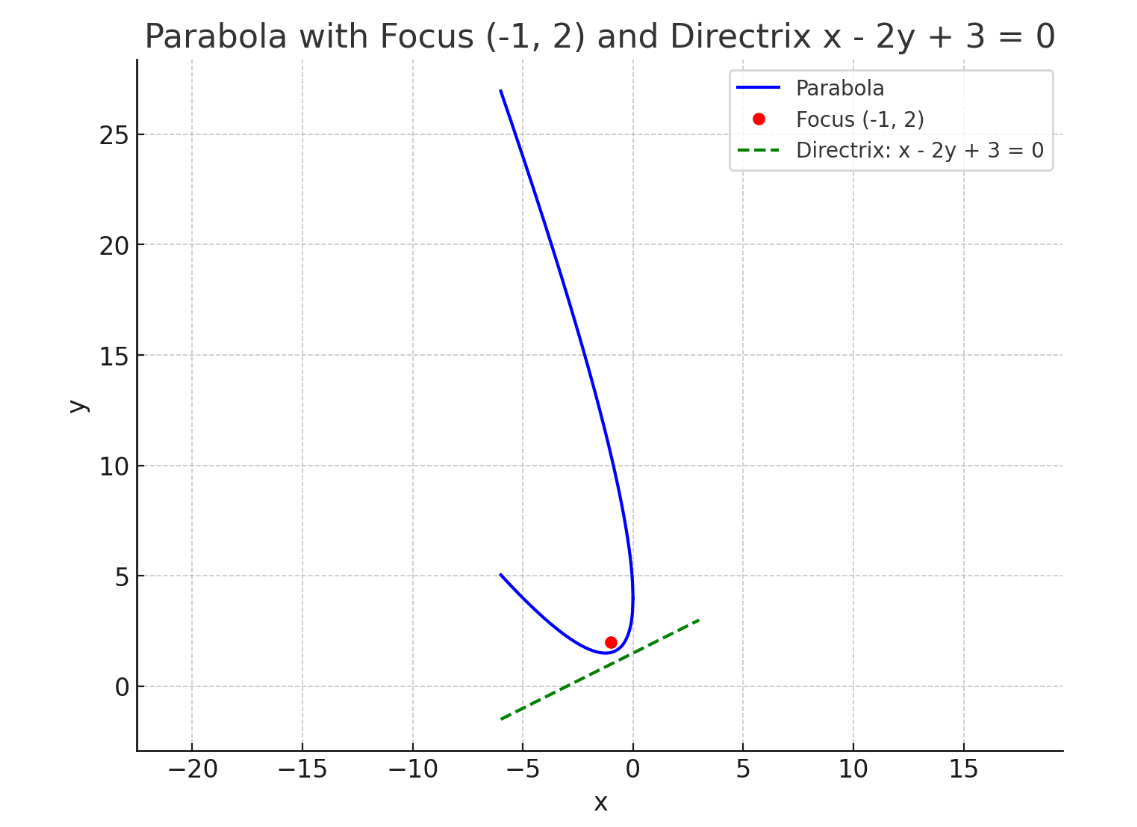
\includegraphics[width=0.85\linewidth]{figs/image.png}
        \caption{Image}
        \label{fig:placeholder}
    \end{figure}
\end{frame}

\begin{frame}[fragile]{C code}
    \begin{lstlisting}
        #include <stdio.h>
#include <math.h>

int main() {
    // Define vectors and constants
    double F[2] = {-1, 2};      // Focus
    double n[2] = {1, -2};      // Normal vector to directrix
    double c = -3;              // Constant term from directrix n^T x = c
    double e = 1;               // Parabola => e = 1
    // Compute ||n||^2
    double norm_n2 = n[0]*n[0] + n[1]*n[1];
    // Identity matrix I
    double I[2][2] = {{1, 0}, {0, 1}};
    // Compute n*n^T
    double nnT[2][2];
    for(int i=0; i<2; i++)
        for(int j=0; j<2; j++)
            nnT[i][j] = n[i]*n[j];
    \end{lstlisting}
\end{frame}

\begin{frame}[fragile]{C code}
    \begin{lstlisting}
         // Compute V = ||n||^2 * I - e^2 * (n*n^T)
    double V[2][2];
    for(int i=0; i<2; i++)
        for(int j=0; j<2; j++)
            V[i][j] = norm_n2*I[i][j] - e*e*nnT[i][j];

    // Compute u = c*e^2*n - ||n||^2 * F
    double u[2];
    for(int i=0; i<2; i++)
        u[i] = c*e*e*n[i] - norm_n2*F[i];

    // Compute f = ||n||^2 * ||F||^2 - c^2 * e^2
    double f = norm_n2 * (F[0]*F[0] + F[1]*F[1]) - (c*c*e*e);

    // Display results
    printf("Matrix Form of Parabola:\n\n");

    printf("V = [ [%.2f, %.2f], [%.2f, %.2f] ]\n",
           V[0][0], V[0][1], V[1][0], V[1][1]);
    \end{lstlisting}
\end{frame}

\begin{frame}[fragile]{C code}
    \begin{lstlisting}
        printf("u = [ %.2f, %.2f ]^T\n", u[0], u[1]);
    printf("f = %.2f\n\n", f);

    printf("Conic Equation: x^T V x + 2u^T x + f = 0\n");
    printf("=> [x y] [%.2f %.2f; %.2f %.2f] [x; y] + 2[%.2f %.2f][x; y] + %.2f = 0\n",
           V[0][0], V[0][1], V[1][0], V[1][1], u[0], u[1], f);

    return 0;
}
    \end{lstlisting}
\end{frame}

\begin{frame}[fragile]{Python code}
    \begin{lstlisting}
        import numpy as np
import matplotlib.pyplot as plt

# Parabola equation from matrix form:
# 4x² + 4xy + y² + 4x - 8y + 16 = 0
# We'll use this to plot the curve.

# Define grid
x = np.linspace(-8, 6, 400)
y = np.linspace(-4, 8, 400)
X, Y = np.meshgrid(x, y)

# Define the equation of the parabola
F = 4*X**2 + 4*X*Y + Y**2 + 4*X - 8*Y + 16

# Plot the parabola (F=0)
plt.contour(X, Y, F, levels=[0], colors='b', linewidths=2, label='Parabola')
    \end{lstlisting}
\end{frame}

\begin{frame}[fragile]{C code}
    \begin{lstlisting}
        # Plot directrix: x - 2y + 3 = 0  →  y = (x + 3)/2
x_dir = np.linspace(-8, 6, 200)
y_dir = (x_dir + 3) / 2
plt.plot(x_dir, y_dir, 'g--', label='Directrix')

# Focus point (-1, 2)
plt.plot(-1, 2, 'ro', label='Focus (-1, 2)')

# Graph settings
plt.axis('equal')
plt.grid(True, linestyle='--', alpha=0.6)
plt.title('Parabola with Focus (-1, 2) and Directrix x - 2y + 3 = 0')
plt.xlabel('x-axis')
plt.ylabel('y-axis')
plt.legend()
plt.show()
    \end{lstlisting}
\end{frame}

\end{document}